%%
%% This is file `tikzposter-template.tex',
%% generated with the docstrip utility.
%%
%% The original source files were:
%%
%% tikzposter.dtx  (with options: `tikzposter-template.tex')
%%
%% This is a generated file.
%%
%% Copyright (C) 2014 by Pascal Richter, Elena Botoeva, Richard Barnard, and Dirk Surmann
%%
%% This file may be distributed and/or modified under the
%% conditions of the LaTeX Project Public License, either
%% version 2.0 of this license or (at your option) any later
%% version. The latest version of this license is in:
%%
%% http://www.latex-project.org/lppl.txt
%%
%% and version 2.0 or later is part of all distributions of
%% LaTeX version 2013/12/01 or later.
%%


\documentclass{tikzposter} %Options for format can be included here

\usepackage{todonotes}

\usepackage[tikz]{bclogo}
\usepackage{lipsum}
\usepackage{amsmath}

\usepackage{booktabs}
\usepackage{longtable}
\usepackage[absolute]{textpos}
\usepackage[it]{subfigure}
\usepackage{graphicx}
\usepackage{cmbright}
%\usepackage[default]{cantarell}
%\usepackage{avant}
%\usepackage[math]{iwona}
\usepackage[math]{kurier}
\usepackage[T1]{fontenc}


%% add your packages here
\usepackage{hyperref}
% for random text
\usepackage{lipsum}
\usepackage[english]{babel}
\usepackage[pangram]{blindtext}

\colorlet{backgroundcolor}{blue!10}

 % Title, Author, Institute
\title{TMDB Box Office Prediction}
\author{Shukai Wang}
\institute{ Xi'an Shiyou University, China \\
}
%\titlegraphic{logos/tulip-logo.eps}

%Choose Layout
\usetheme{Wave}

%\definebackgroundstyle{samplebackgroundstyle}{
%\draw[inner sep=0pt, line width=0pt, color=red, fill=backgroundcolor!30!black]
%(bottomleft) rectangle (topright);
%}
%
%\colorlet{backgroundcolor}{blue!10}

\begin{document}


\colorlet{blocktitlebgcolor}{blue!23}

 % Title block with title, author, logo, etc.
\maketitle

\begin{columns}
 % FIRST column
\column{0.5}% Width set relative to text width

%%%%%%%%%% -------------------------------------------------------------------- %%%%%%%%%%
 %\block{Main Objectives}{
%  	      	\begin{enumerate}
%  	      	\item Formalise research problem by extending \emph{outlying aspects mining}
%  	      	\item Proposed \emph{GOAM} algorithm is to solve research problem
%  	      	\item Utilise pruning strategies to reduce time complexity
%  	      	\end{enumerate}
%%  	      \end{minipage}
%}
%%%%%%%%%% -------------------------------------------------------------------- %%%%%%%%%%


%%%%%%%%%% -------------------------------------------------------------------- %%%%%%%%%%
\block{Introduction}{
  "In 2018, film revenue has increased significantly, and the film industry is more popular than ever. 
   What kind of movies make high box office receipts. In the process of preparation and shooting, 
   whether the budget, the number of directors and actors have a great impact. Whether the publicity and 
   preview of later films will affect the final box office income of films.
  	
  	\begin{description}
    \item[Data Analysis] aims to show the relationship between attributes and 
    box office revenue according to the data provided. And further integration of data, 
    delete irrelevant data, unified data values and so on.
  	
    \item[Models and Forecasts] aims to use the integrated data to train the relevant models, 
    improve the accuracy, and make the box office revenue forecast for some of the given data.
  	\end{description}

  	In this paper,
    we train the random forest model with the integrated data, 
    and use the model to predict the box office of movies.
}
%%%%%%%%%% -------------------------------------------------------------------- %%%%%%%%%%


%%%%%%%%%% -------------------------------------------------------------------- %%%%%%%%%%
\block{Data Analysis}{
\begin{itemize}
    \item
    %\emph{Group Outlying Aspects Mining}
    In the pre production budget, the number of actors and the number of 
    directors and other crew members on the impact of box office.
\end{itemize}

\begin{center}
    \begin{minipage}{0.3\linewidth}
    \centering
    \begin{tikzfigure}
      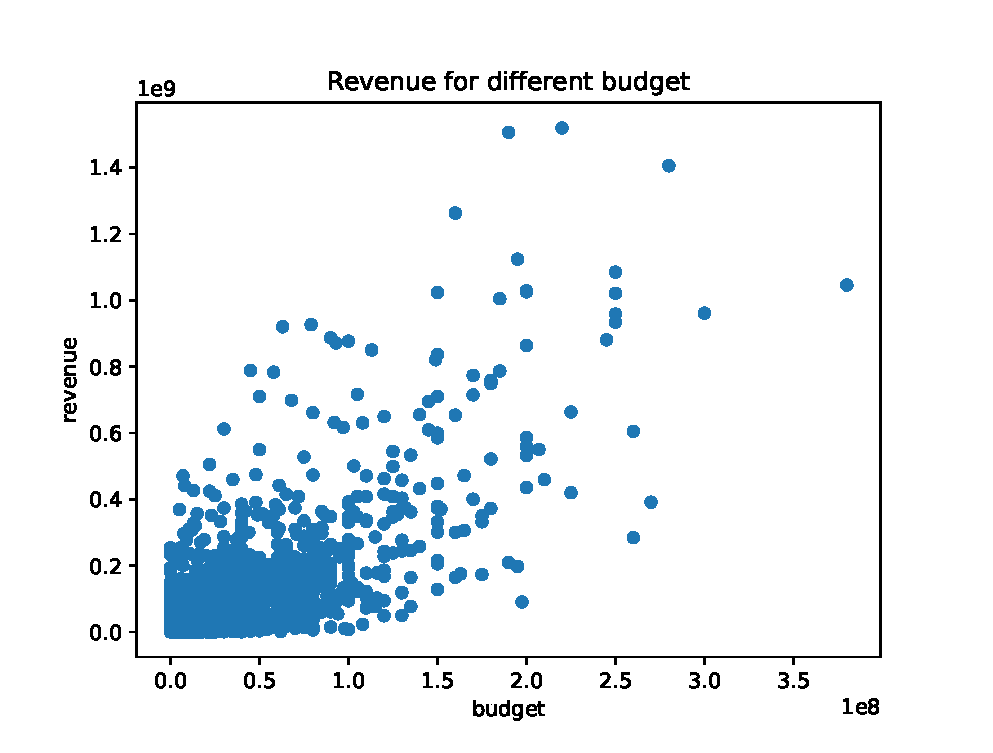
\includegraphics[width=0.8\linewidth]{figures//budget.eps}
    {\small{Budget}}
    \end{tikzfigure}%
    \end{minipage}
    \hfill
    \begin{minipage}{0.3\linewidth}
    \centering
    \begin{tikzfigure}
      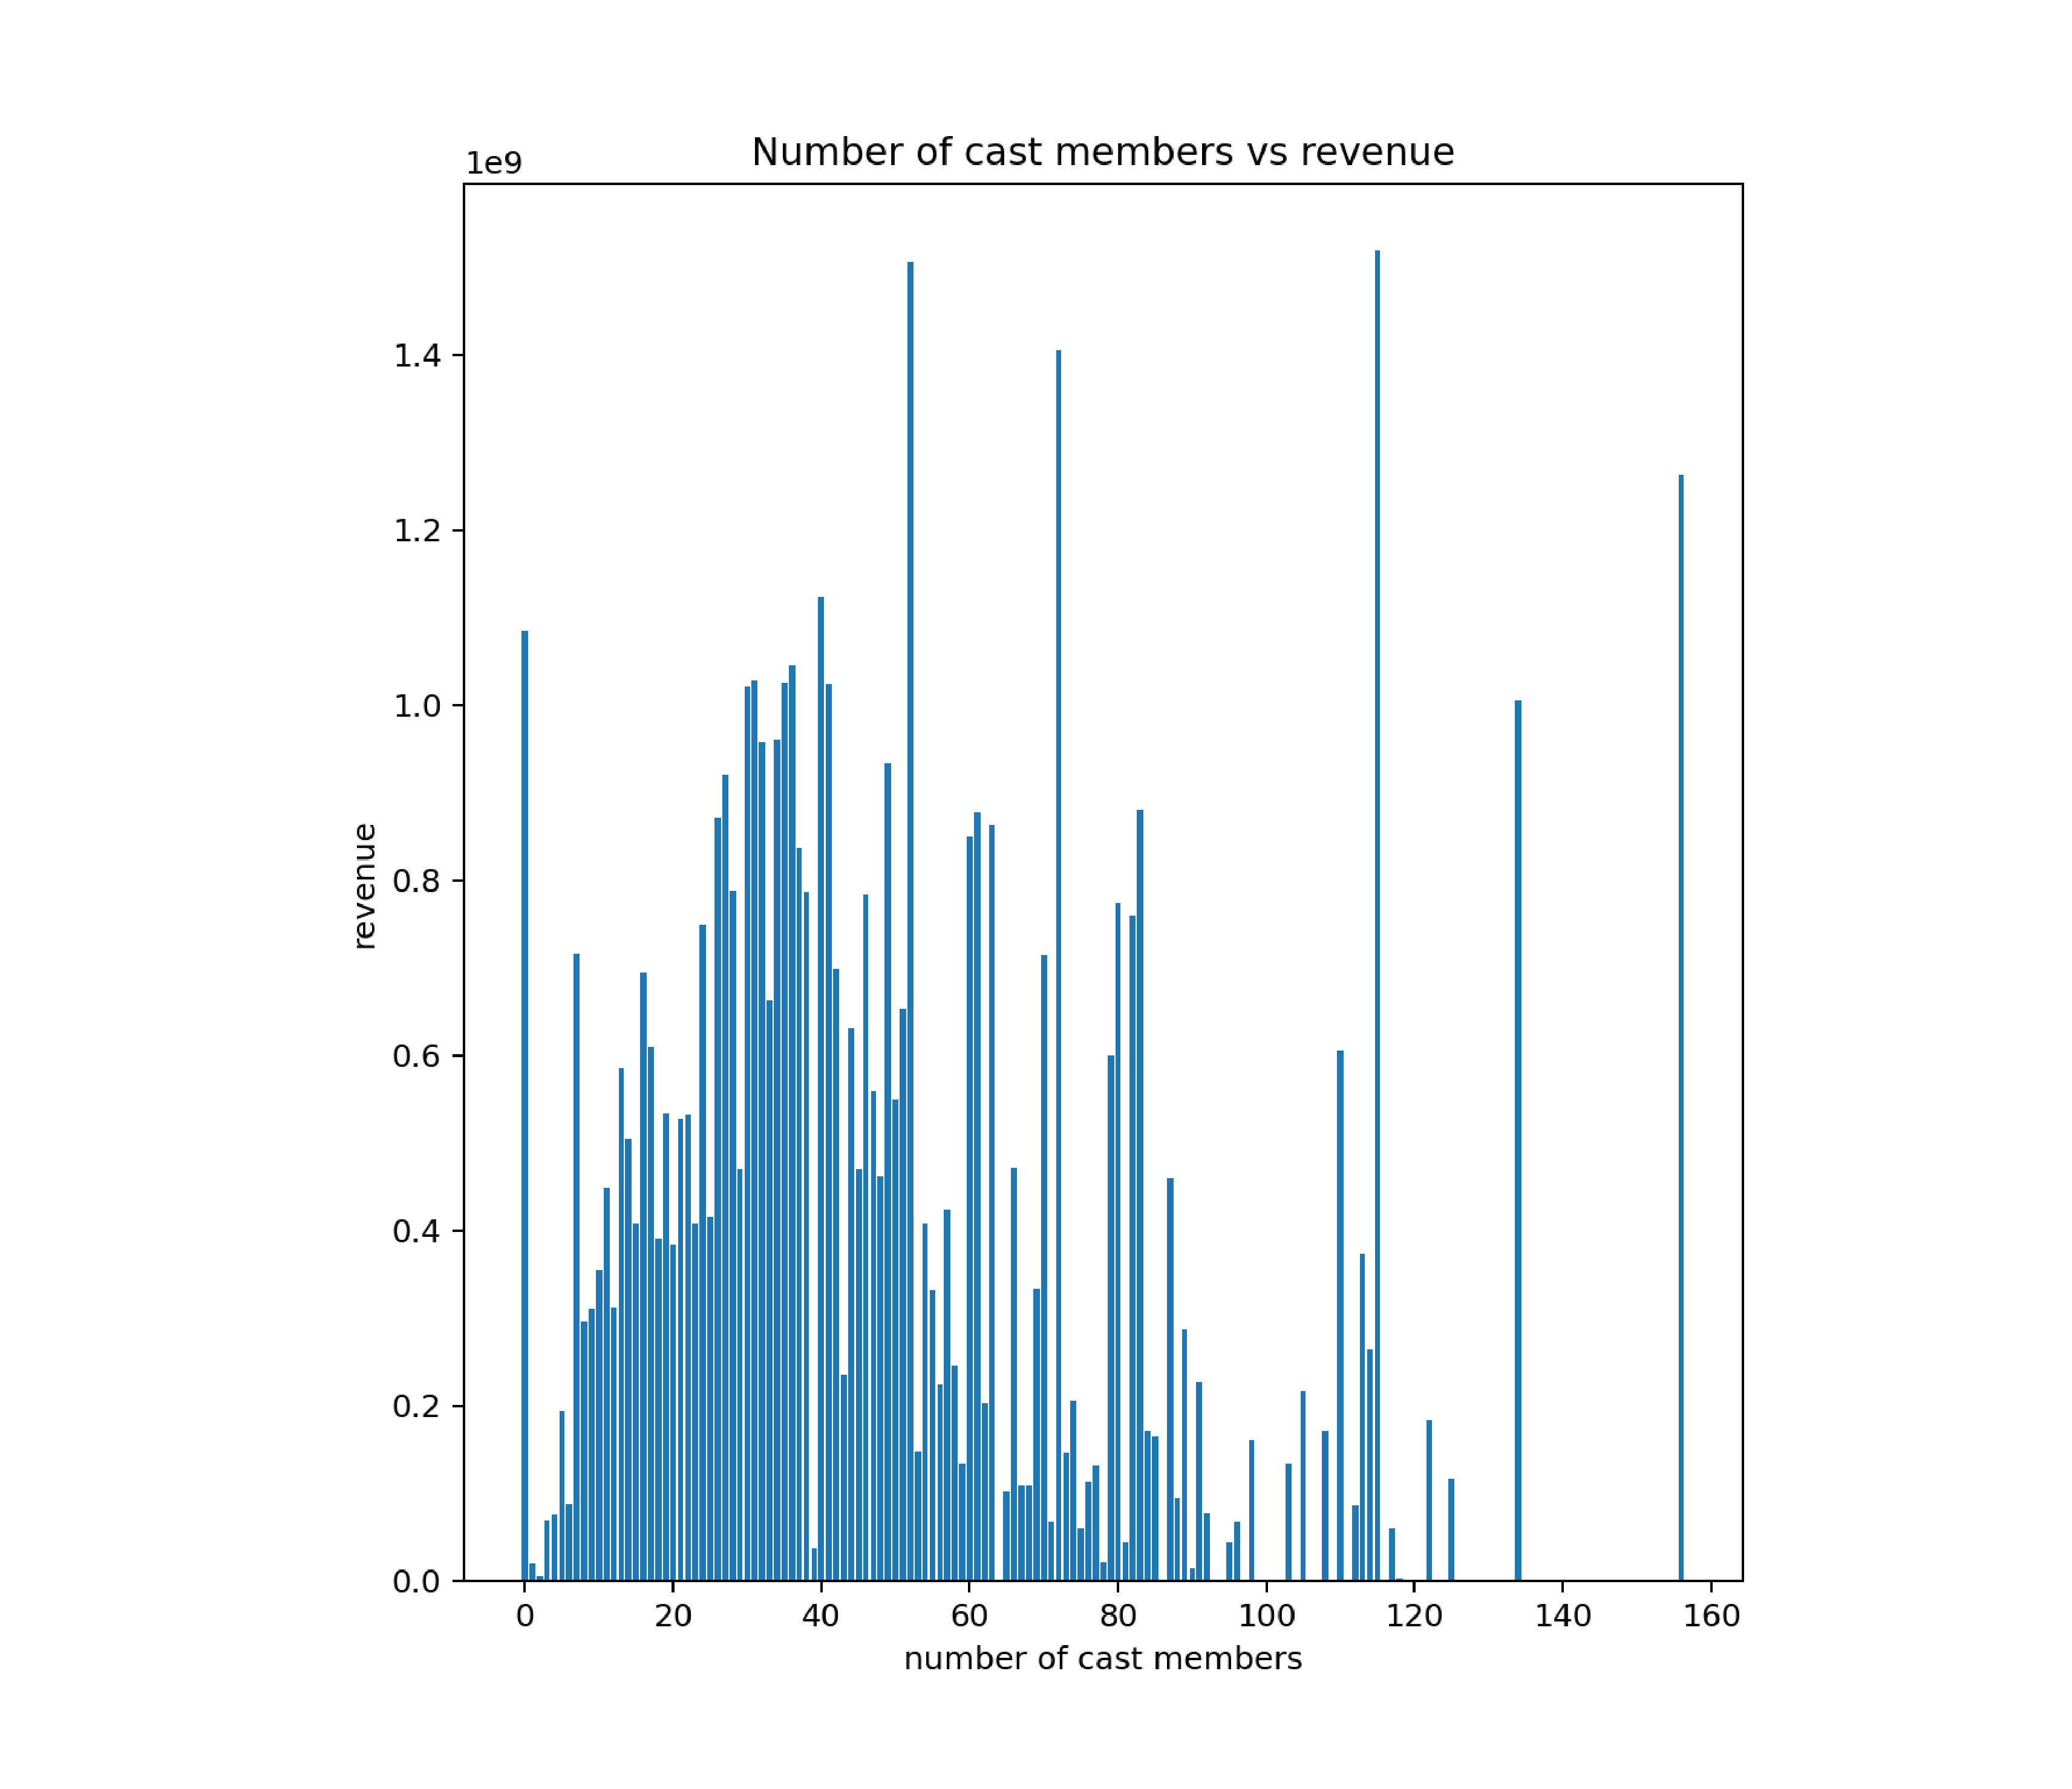
\includegraphics[width=0.8\linewidth]{figures//cest.eps}\\
    {\small{Cast}}
    \end{tikzfigure}%
    \end{minipage}
    \hfill
    \begin{minipage}{0.3\linewidth}
    \centering
    \begin{tikzfigure}
      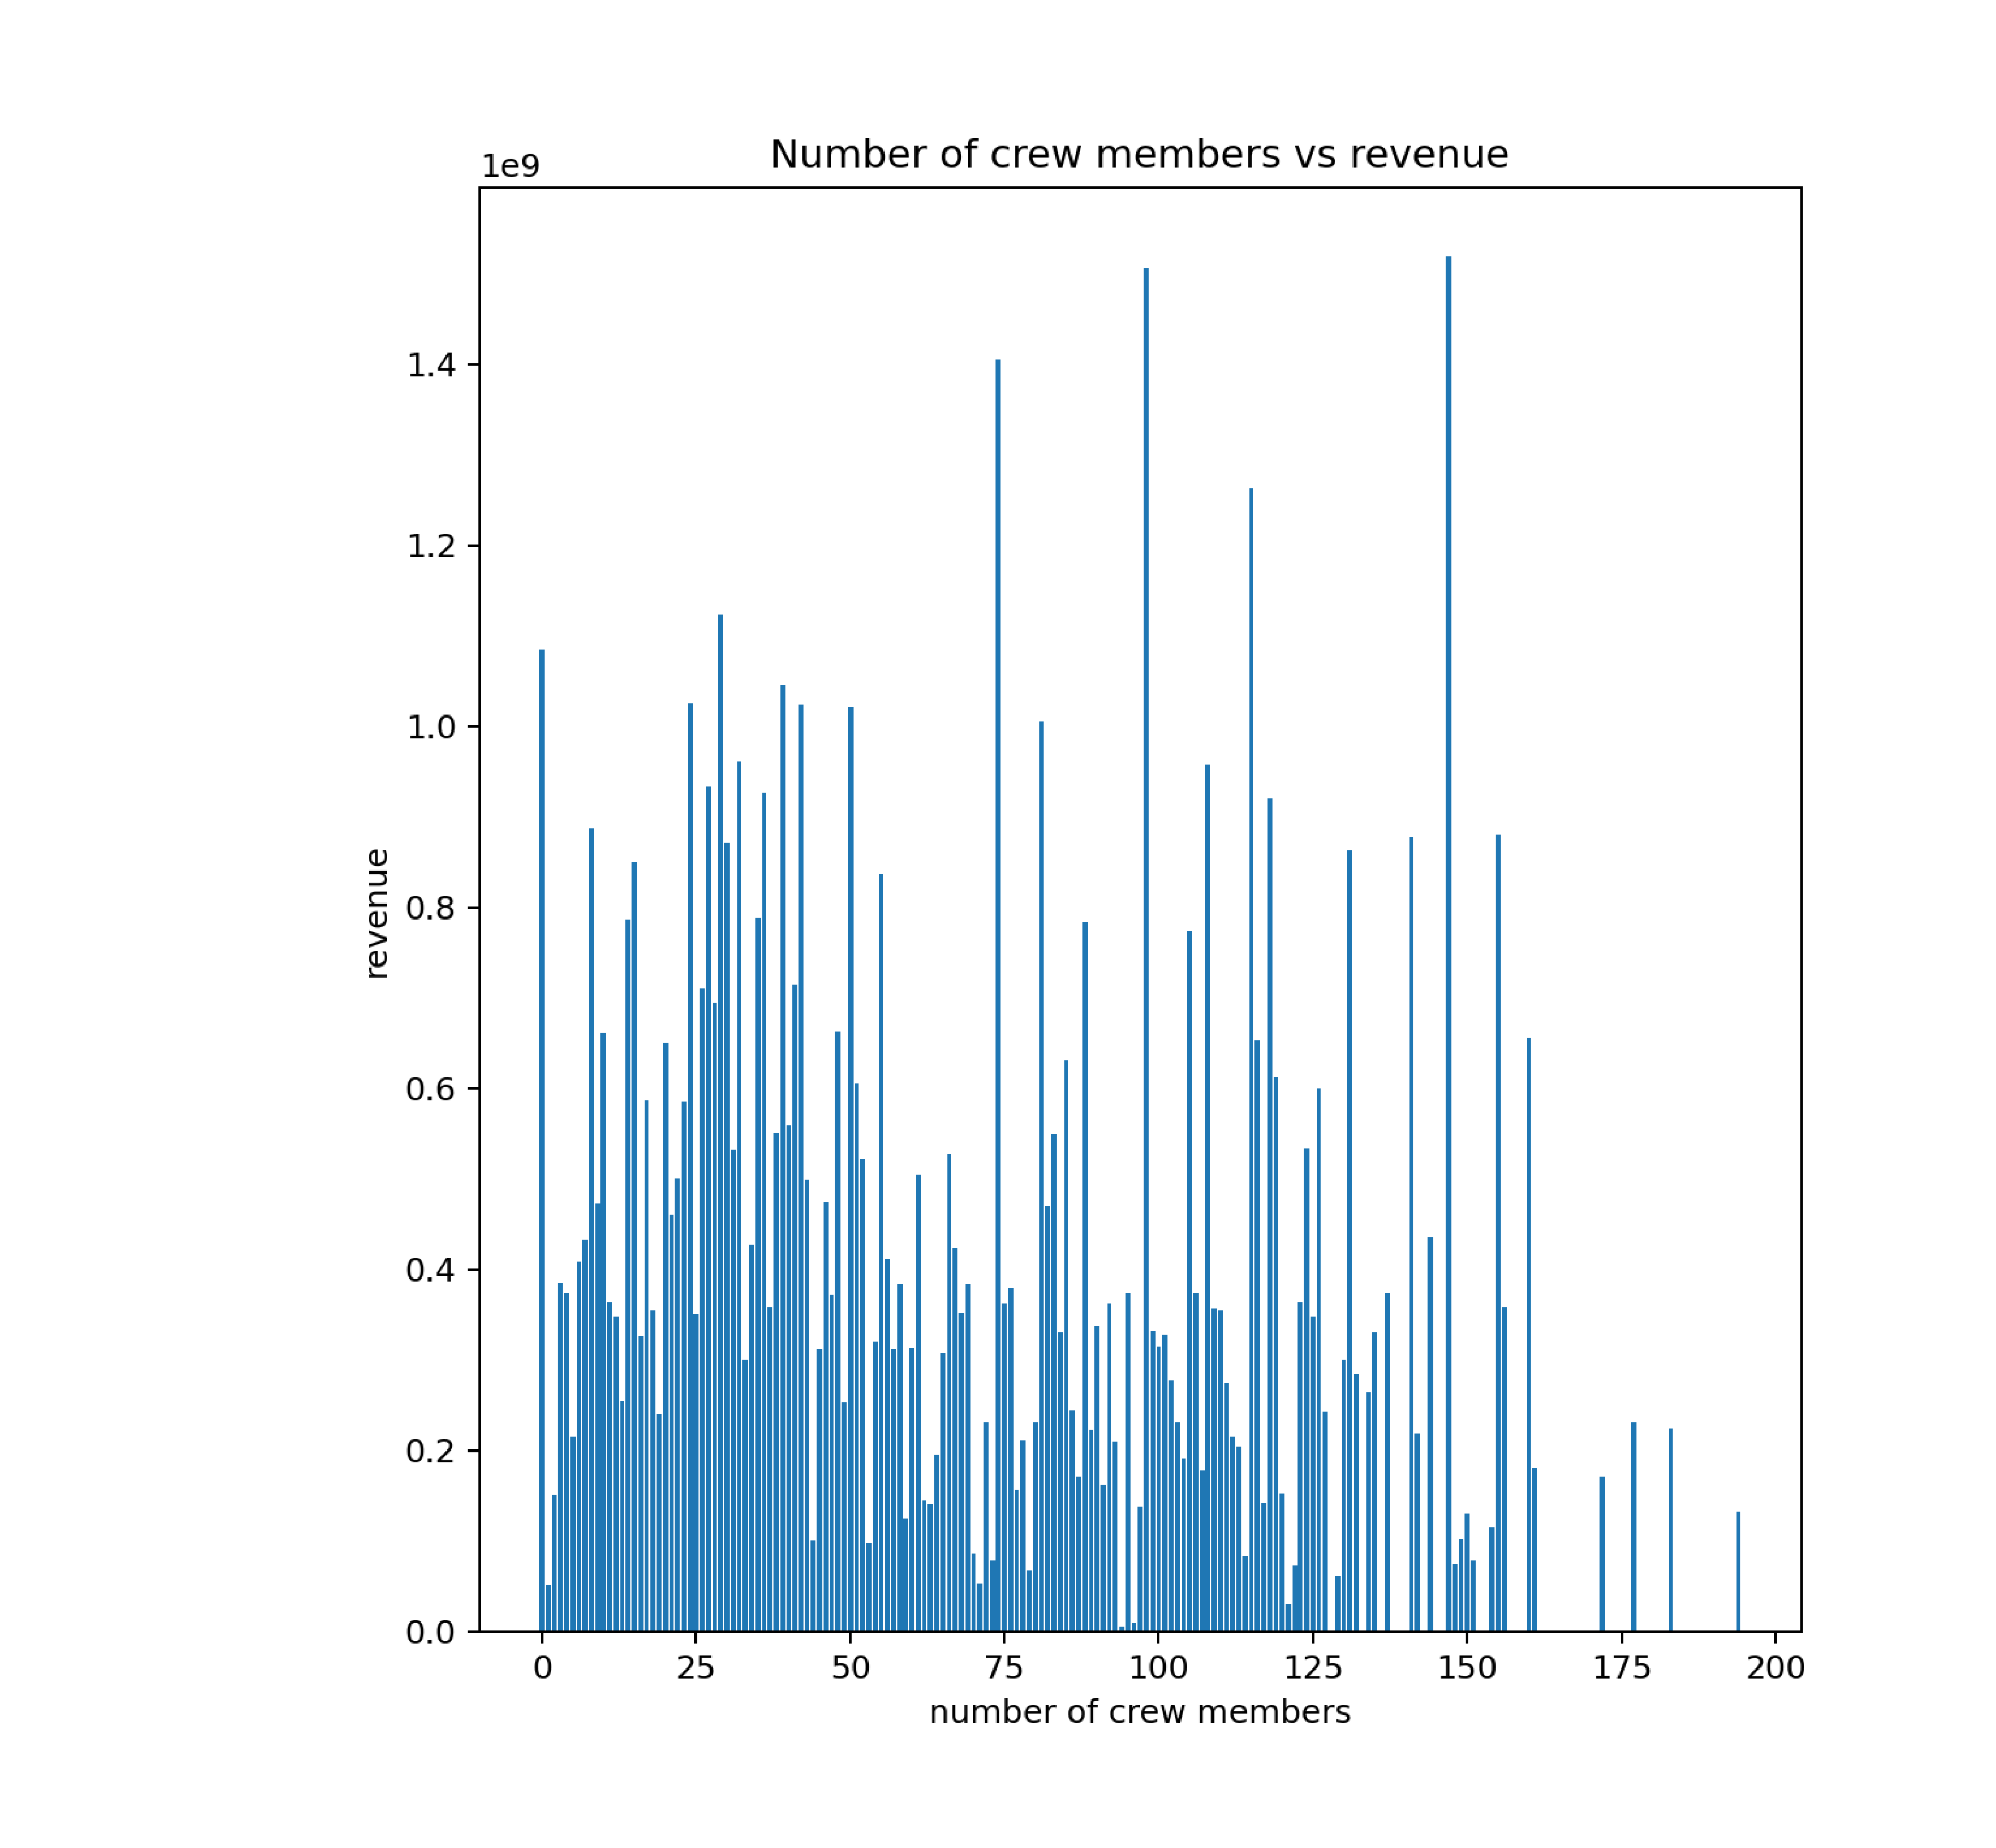
\includegraphics[width=0.8\linewidth]{figures//crew.eps}\\
    {\small{Crew}}
    \end{tikzfigure}%
    \end{minipage}
\end{center}

\begin{itemize}
  \item
  %\emph{Group Outlying Aspects Mining}
  In the late stage of film production, the influence of home page, 
  film introduction, film tagline on the box office of films is also discussed.
\end{itemize}

\begin{center}
  \begin{minipage}{0.3\linewidth}
  \centering
  \begin{tikzfigure}
    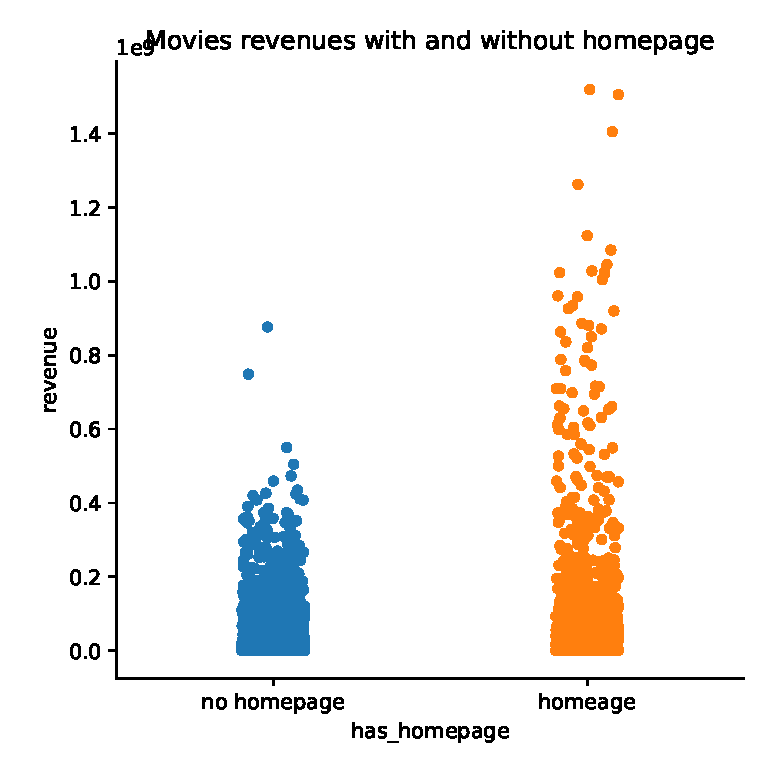
\includegraphics[width=0.8\linewidth]{figures//has_homepage.eps}
  {\small{Homepage}}
  \end{tikzfigure}%
  \end{minipage}
  \hfill
  \begin{minipage}{0.3\linewidth}
  \centering
  \begin{tikzfigure}
    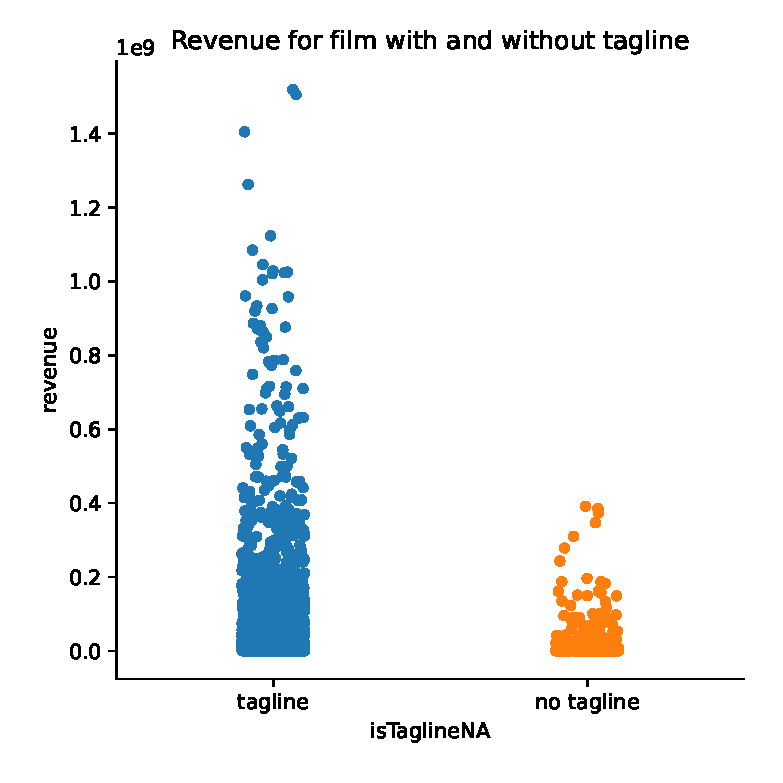
\includegraphics[width=0.8\linewidth]{figures//isTanglineNA.eps}
  {\small{Tagline}}
  \end{tikzfigure}%
  \end{minipage}
  \hfill
  \begin{minipage}{0.3\linewidth}
  \centering
  \begin{tikzfigure}
    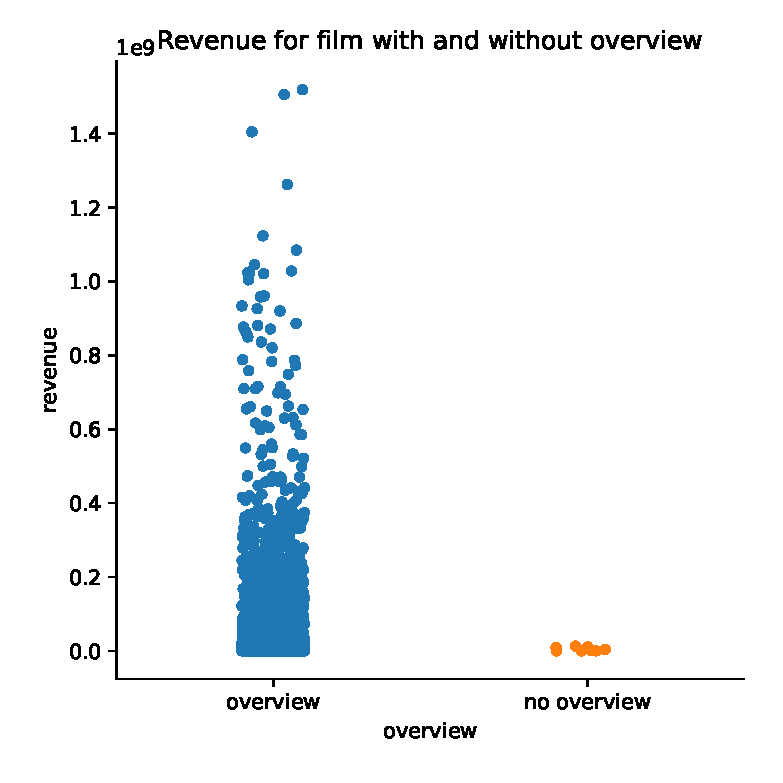
\includegraphics[width=0.8\linewidth]{figures//overview.eps}
  {\small{Overview}}
  \end{tikzfigure}%
  \end{minipage}
\end{center}

\begin{itemize}
  \item
  %\emph{Group Outlying Aspects Mining}
  Some other influences, such as film series, 
  film companies and the number of film companies participating in the investment, etc.
\end{itemize}

\begin{center}
  \begin{minipage}{0.3\linewidth}
  \centering
  \begin{tikzfigure}
    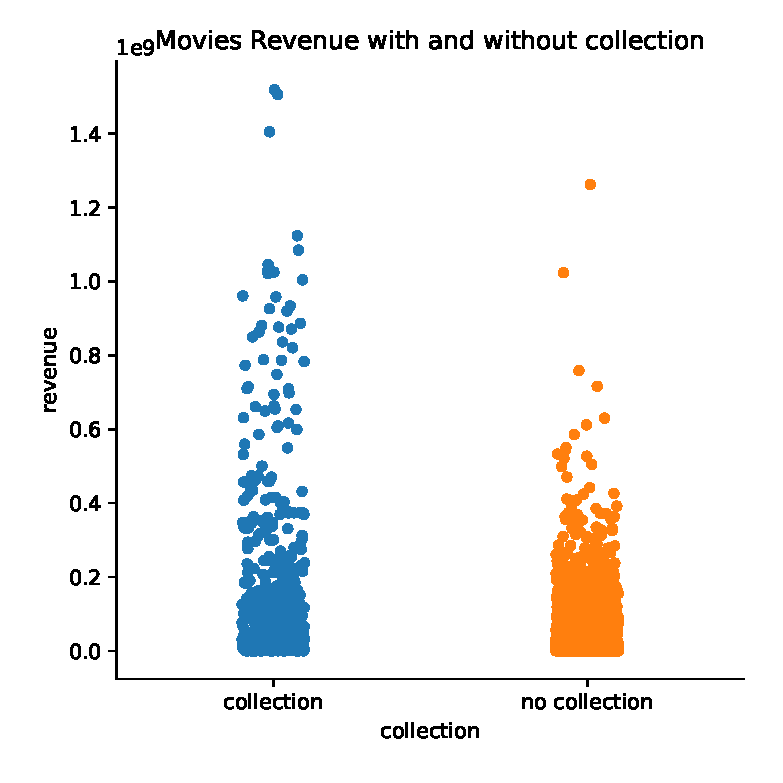
\includegraphics[width=0.8\linewidth]{figures//collection.eps}
  {\small{File Series}}
  \end{tikzfigure}%
  \end{minipage}
  \hfill
  \begin{minipage}{0.3\linewidth}
  \centering
  \begin{tikzfigure}
    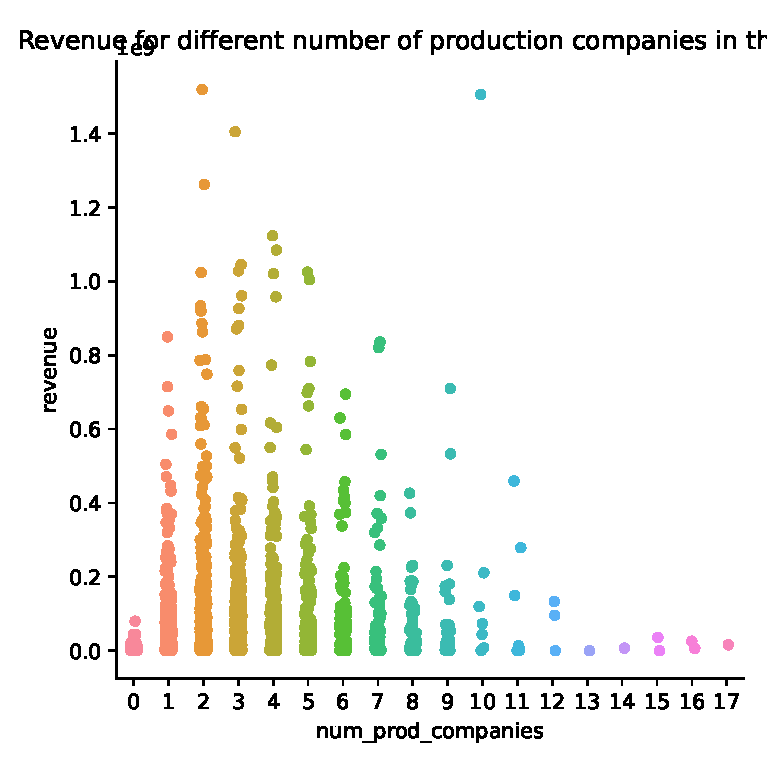
\includegraphics[width=0.8\linewidth]{figures//company.eps}
  {\small{File Company}}
  \end{tikzfigure}%
  \end{minipage}
  \hfill
  \begin{minipage}{0.3\linewidth}
  \centering
  \begin{tikzfigure}
    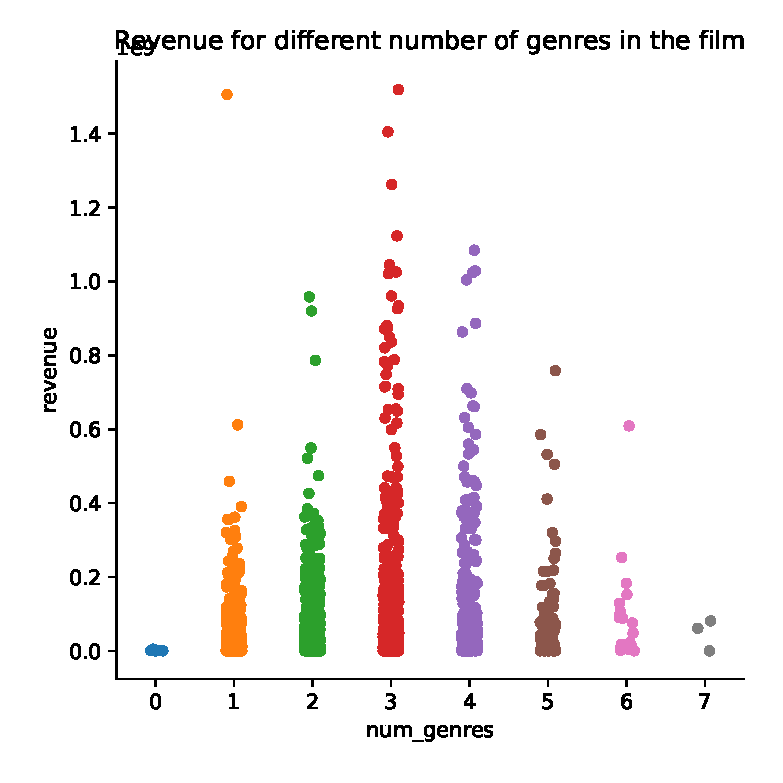
\includegraphics[width=0.8\linewidth]{figures//counrty.eps}
  {\small{Company Number}}
  \end{tikzfigure}%
  \end{minipage}
\end{center}

\begin{itemize}
  \item
  %\emph{Group Outlying Aspects Mining}
  The popularity of the film's language and genre among 
  the audience also affects the box office.
\end{itemize}

\begin{center}
  \begin{minipage}{0.4\linewidth}
  \centering
  \begin{tikzfigure}
    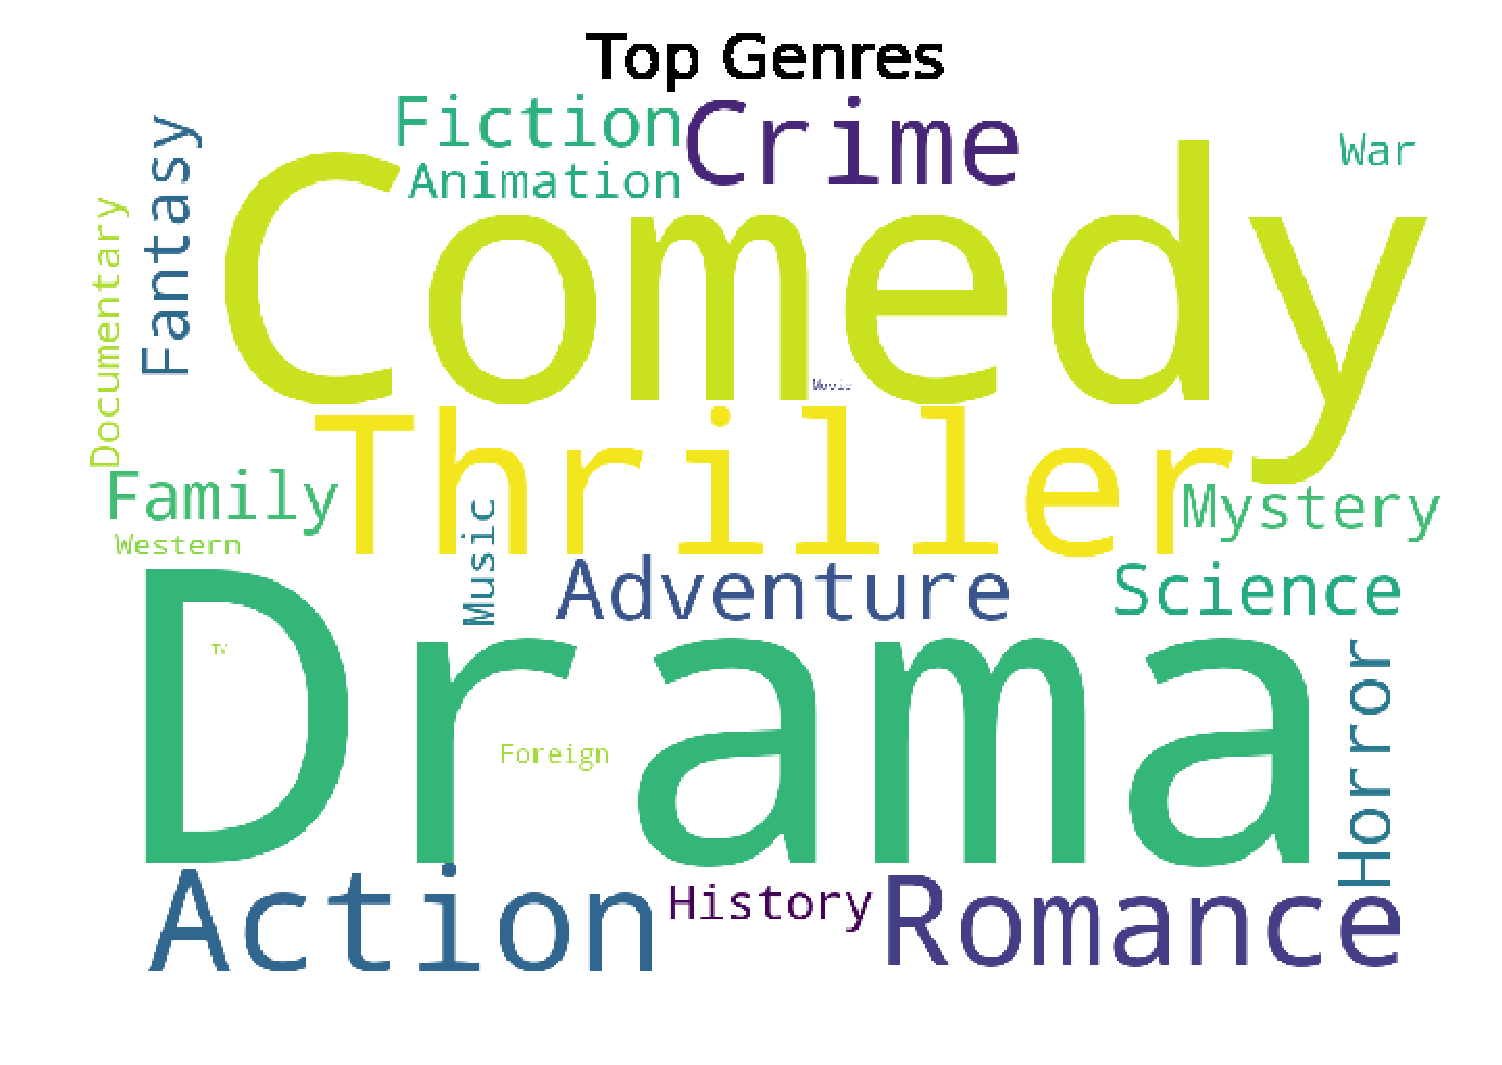
\includegraphics[width=0.8\linewidth]{figures//genre_clold.eps}\\
  {\small{Genre}}
  \end{tikzfigure}%
  \end{minipage}
  \hfill
  \begin{minipage}{0.4\linewidth}
  \centering
  \begin{tikzfigure}
    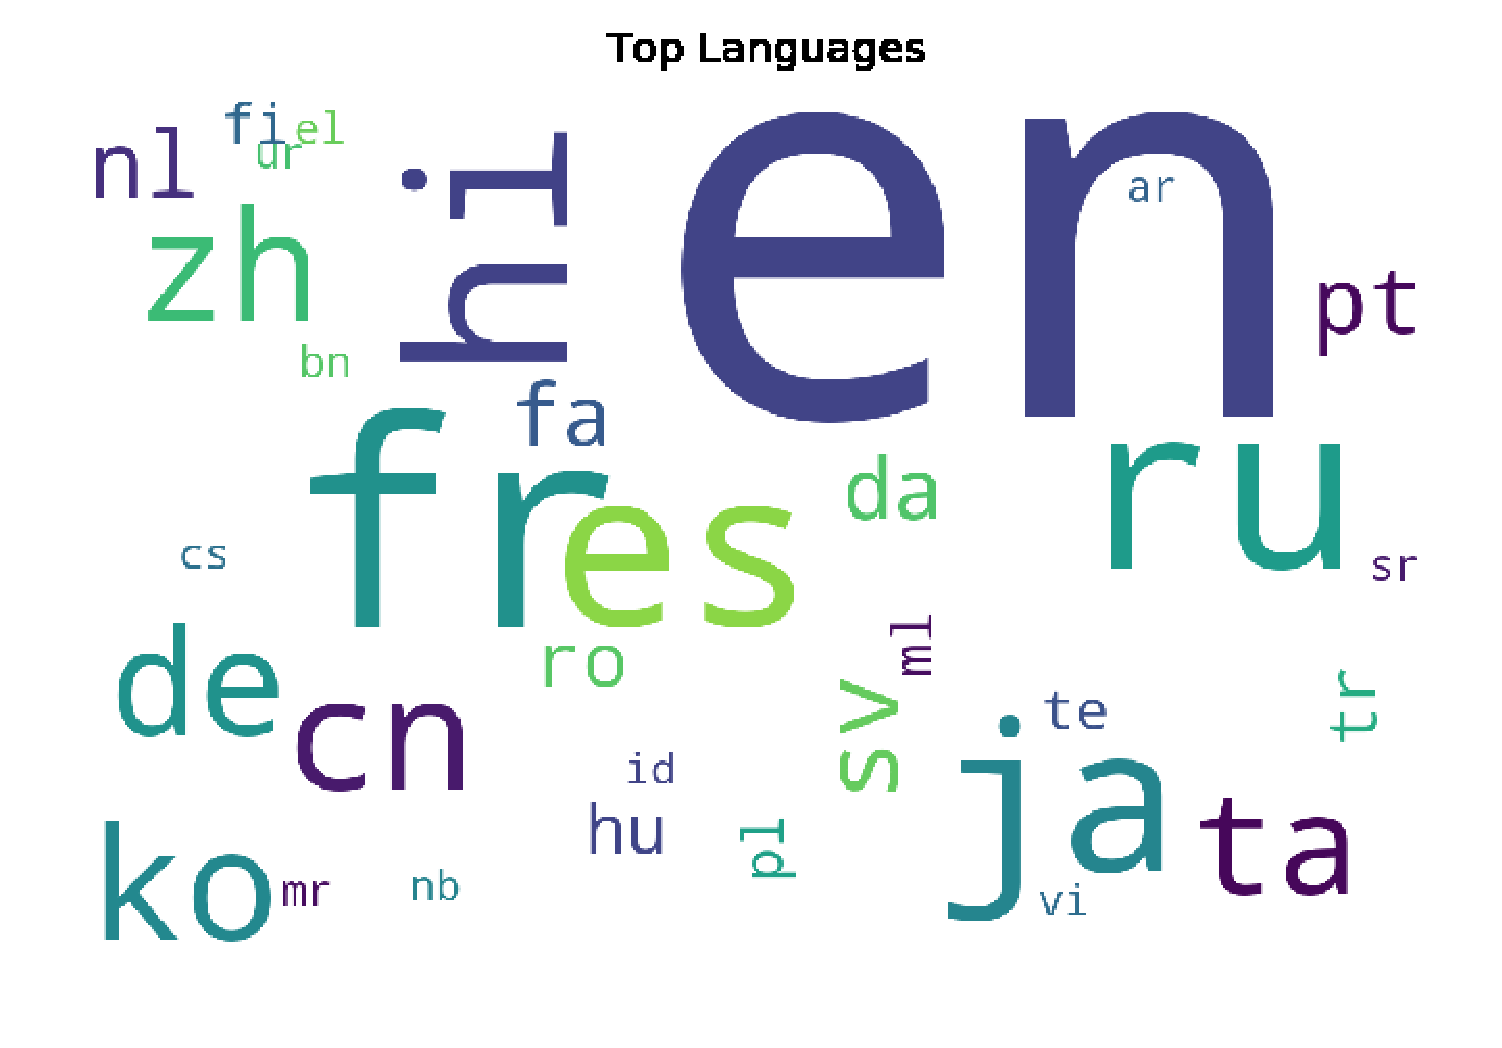
\includegraphics[width=0.8\linewidth]{figures//language.eps}\\
  {\small{Language}}
  \end{tikzfigure}%
  \end{minipage}
  \hfill
  
\end{center}

}
%%%%%%%%%% -------------------------------------------------------------------- %%%%%%%%%%


%%%%%%%%%% -------------------------------------------------------------------- %%%%%%%%%%

%\note{Note with default behavior}

%\note[targetoffsetx=12cm, targetoffsety=-1cm, angle=20, rotate=25]
%{Note \\ offset and rotated}

 % First column - second block


%%%%%%%%%% -------------------------------------------------------------------- %%%%%%%%%%


% SECOND column
\column{0.5}
 %Second column with first block's top edge aligned with with previous column's top.

%%%%%%%%%% -------------------------------------------------------------------- %%%%%%%%%%
\block{Data Processing}{
  \begin{itemize}
    \item Processing data that does not affect the box office.
  \end{itemize}
  \\  
  \begin{tabular}{ c | c }
      \toprule
      Name     &  Description        \\
      \midrule
      imdb id       &  ID of movie in TMDB  \\
      orginal title &  The original name of the movie \\
      poster path &  Movie poster link \\
      status   & The state of the film \\
      \bottomrule
  \end{tabular}
  \\
  \begin{itemize}
    \item Normalized training data and test data.
  \end{itemize}\\

  \begin{tabular}{ c | c }
      \toprule
      Name     &  Description        \\
      \midrule
      keywords      &  Key words of movies \\
      tagline &  The slogan of the film \\
      homepage & Official film Homepage \\
      overview   &A brief description of the film \\
      collection & Series name of film series\\
      release date & Film release time\\ 
      \bottomrule
  \end{tabular}
}
%%%%%%%%%% -------------------------------------------------------------------- %%%%%%%%%%
% Second column - first block


%%%%%%%%%% -------------------------------------------------------------------- %%%%%%%%%%
\block[titleleft]{Model}
{
\begin{description}
  	\item[Random Forest Algorithm] is an ensemble technique that combines multiple decision trees. 
    Other advantages of random forests are that they are less sensitive to outliers in the dataset 
    and don’t require much parameter tuning.  
\end{description}
    \begin{itemize}
      \item Accuracy:2.21274632296787
    \end{itemize}
\begin{description}
    \item[Linear Regression] is a statistical analysis method that uses regression analysis in 
    mathematical statistics to determine the quantitative relationship between two or more variables, 
    which is often fitted by least square approximation.
\end{description}
\begin{itemize}
  \item Accuracy:2.4236034243650315
\end{itemize}

}
%%%%%%%%%% -------------------------------------------------------------------- %%%%%%%%%%

\block[titleleft]{Forecast}
{
  The accuracy of linear regression is higher than that of linear regression.
  Random forest was selected for prediction.

\begin{itemize}
  \item Random forest algorithm for prediction
\end{itemize}

\begin{tabular}{ p{100pt} | p{250pt} }
  \toprule
  id & revenue\\
  \midrule
  3001 & 193077.0567 \\
  3002 &  528484.58  \\
  3003 &  4562948.933\\
  3004 & 14433891.04\\
  3005 &  494782.0824 \\
  3006 &  3010483.492 \\
  3007 &  2100402.514 \\
  3008 &  37411400.18 \\
  \bottomrule
\end{tabular}
}

% Second column - second block
%%%%%%%%%% -------------------------------------------------------------------- %%%%%%%%%%
\block[titlewidthscale=1, bodywidthscale=1]
{Conclusion}
{
  \begin{itemize}
    \item The investment in the early stage and publicity in the later stage have an impact on the box office.
    \item In the early stage, the number of actors and crew should be moderate, not the more the better.
    \item The prediction accuracy can be further \\improved, such as using XGBoost.
  \end{itemize}
}
%%%%%%%%%% -------------------------------------------------------------------- %%%%%%%%%%


% Bottomblock
%%%%%%%%%% -------------------------------------------------------------------- %%%%%%%%%%
\colorlet{notebgcolor}{blue!20}
\colorlet{notefrcolor}{blue!20}
\note[targetoffsetx=8cm, targetoffsety=-4cm, angle=30, rotate=15,
radius=2cm, width=.26\textwidth]{
Acknowledgement
\begin{itemize}
    \item 
    Flip00,TULIP Group
    %International Cooperation Project (Y7Z0511101)
    %of IIE,
    %Chinese Academy of Sciences
 \end{itemize}
}

%\note[targetoffsetx=8cm, targetoffsety=-10cm,rotate=0,angle=180,radius=8cm,width=.46\textwidth,innersep=.1cm]{
%Acknowledgement
%}

%\block[titlewidthscale=0.9, bodywidthscale=0.9]
%{Acknowledgement}{
%}
%%%%%%%%%% -------------------------------------------------------------------- %%%%%%%%%%

\end{columns}


%%%%%%%%%% -------------------------------------------------------------------- %%%%%%%%%%
%[titleleft, titleoffsetx=2em, titleoffsety=1em, bodyoffsetx=2em,%
%roundedcorners=10, linewidth=0mm, titlewidthscale=0.7,%
%bodywidthscale=0.9, titlecenter]

%\colorlet{noteframecolor}{blue!20}
\colorlet{notebgcolor}{blue!20}
\colorlet{notefrcolor}{blue!20}
\note[targetoffsetx=-13cm, targetoffsety=-12cm,rotate=0,angle=180,radius=8cm,width=.96\textwidth,innersep=.4cm]
{
\begin{minipage}{0.3\linewidth}
\centering

\includegraphics[width=24cm]{logos/tulip-wordmark.eps}
\end{minipage}
\begin{minipage}{0.7\linewidth}
{ \centering

% The $11^{th}$ International Conference on Knowledge Science,
%  Engineering and Management (KSEM 2018),
 % 17-19/08/2018, Changchun, China
}
\end{minipage}
}
%%%%%%%%%% -------------------------------------------------------------------- %%%%%%%%%%


\end{document}

%\endinput
%%
%% End of file `tikzposter-template.tex'.
